\documentclass[aspectratio=169,10pt]{beamer}

\usepackage[spanish,es-nodecimaldot]{babel}
\usepackage[T1]{fontenc}
\usepackage[utf8]{inputenc}
\usepackage{lmodern}
\usepackage{amsmath,amssymb}
\usepackage{booktabs,array,tabularx,colortbl}
\usepackage{graphicx}
\usepackage{tikz}
\usetikzlibrary{arrows.meta,positioning}

\graphicspath{{docs/informe/assets/}{../informe/assets/}}

\definecolor{paper}{HTML}{FAFAF7}
\definecolor{ink}{HTML}{243746}
\definecolor{navy}{HTML}{FAFAF7}
\definecolor{navytwo}{HTML}{F0F3F5}
\definecolor{navythree}{HTML}{E5EAEE}
\definecolor{teal}{HTML}{2B5F7A}
\definecolor{tealdark}{HTML}{29485C}
\definecolor{amber}{HTML}{856A34}
\definecolor{blue}{HTML}{4F7392}
\definecolor{green}{HTML}{47705D}
\definecolor{red}{HTML}{8C4E4E}
\definecolor{muted}{HTML}{68747D}
\definecolor{border}{HTML}{CBD3D9}
\definecolor{softwhite}{HTML}{FFFFFF}

\setbeamercolor{normal text}{fg=ink,bg=paper}
\setbeamercolor{background canvas}{bg=paper}
\setbeamercolor{structure}{fg=teal}
\setbeamercolor{frametitle}{fg=ink,bg=paper}
\setbeamercolor{footline}{fg=muted,bg=paper}
\setbeamercolor{card}{fg=ink,bg=navytwo}
\setbeamercolor{cardalt}{fg=ink,bg=navythree}
\setbeamercolor{tablehead}{fg=softwhite,bg=tealdark}
\setbeamercolor{tablerow}{fg=ink,bg=navytwo}
\setbeamercolor{tablerowalt}{fg=ink,bg=navythree}

\setbeamertemplate{navigation symbols}{}
\setbeamertemplate{itemize item}{\color{teal}\scriptsize$\bullet$}
\setbeamersize{text margin left=0.65cm,text margin right=0.65cm}

\newcommand{\sectionnamecurrent}{SUSTENTACIÓN}
\newcommand{\speakername}{Equipo MinPol}
\newcommand{\speakertime}{12 minutos}
\newcommand{\sectiontag}[1]{\gdef\sectionnamecurrent{#1}}
\newcommand{\speaker}[2]{\gdef\speakername{#1}\gdef\speakertime{#2}}

\setbeamertemplate{frametitle}{%
  \vspace{0.22cm}%
  {\color{teal}\bfseries\scriptsize\sectionnamecurrent\par}%
  \vspace{0.06cm}%
  {\color{ink}\bfseries\LARGE\insertframetitle\par}%
  \ifx\insertframesubtitle\empty\else
    \vspace{0.02cm}{\color{muted}\small\insertframesubtitle\par}%
  \fi
  \vspace{0.05cm}{\color{border}\rule{\textwidth}{0.4pt}}%
}

\setbeamertemplate{footline}{%
  \leavevmode\hbox{%
    \begin{beamercolorbox}[wd=\paperwidth,ht=0.42cm,dp=0.16cm,leftskip=0.65cm,rightskip=0.65cm]{footline}%
      \bfseries\insertframenumber/\inserttotalframenumber\hspace{0.35cm}\speakername
      \hfill\speakertime\hspace{0.55cm}\textcolor{teal}{\bfseries MinPol}%
    \end{beamercolorbox}}}

\setbeamertemplate{background canvas}[default]

\newcommand{\infocard}[5][card]{%
  \begin{beamercolorbox}[wd=#2,sep=0.22cm]{#1}%
    {\color{#3}\bfseries\large #4}\par\vspace{0.08cm}%
    {\color{ink}#5}%
  \end{beamercolorbox}}

\newcommand{\metric}[3]{%
  \begin{beamercolorbox}[wd=\linewidth,sep=0.14cm,center]{card}%
    {\color{#3}\bfseries\LARGE #1}\par
    {\color{muted}\scriptsize #2}%
  \end{beamercolorbox}}

\newcommand{\pill}[3][teal]{%
  \begin{beamercolorbox}[wd=#2,sep=0.11cm,center]{cardalt}%
    {\color{#1}\bfseries\scriptsize #3}%
  \end{beamercolorbox}}

\begin{document}

% 1. Portada
\sectiontag{SUSTENTACIÓN · ANÁLISIS DE ALGORITMOS II}
\speaker{Juan Carlos Cruz Muñoz}{0:00--0:25}
\begin{frame}[plain]
  \vspace{0.18cm}
  \begin{beamercolorbox}[wd=8.0cm,sep=0.12cm,center,rounded=true]{cardalt}
    {\color{teal}\bfseries\small SUSTENTACIÓN · ANÁLISIS DE ALGORITMOS II}
  \end{beamercolorbox}
  \vspace{0.28cm}
  \begin{columns}[T,onlytextwidth]
    \begin{column}{0.65\textwidth}
      {\fontsize{30}{34}\selectfont\bfseries Minimizar la polarización}\par
      \vspace{0.18cm}
      {\color{muted}\large Un modelo entero lineal para decidir movimientos\\
      bajo presupuesto y distancia limitada}\par
    \end{column}
    \begin{column}{0.30\textwidth}
      \begin{beamercolorbox}[wd=\linewidth,sep=0.35cm,center,rounded=true]{card}
        {\color{teal}\bfseries\LARGE MinPol}\par\vspace{0.16cm}
        {\color{amber}\bfseries\large $\min$}\par\vspace{0.06cm}
        {\bfseries\large $\displaystyle\sum_i y_i|v_i-\operatorname{med}(y)|$}\par
        \vspace{0.18cm}{\color{muted}\small $ct$ · $maxM$ · población}
      \end{beamercolorbox}
    \end{column}
  \end{columns}
  \vspace{0.28cm}
  {\color{teal}\bfseries\small INTEGRANTES}\par\vspace{0.10cm}
  \begin{columns}[T,onlytextwidth]
    \begin{column}{0.49\textwidth}
      \begin{beamercolorbox}[wd=\linewidth,sep=0.13cm,rounded=true]{card}
        \bfseries\small Juan Carlos Cruz Muñoz \hfill 1824389
      \end{beamercolorbox}\vspace{0.10cm}
      \begin{beamercolorbox}[wd=\linewidth,sep=0.13cm,rounded=true]{card}
        \bfseries\small Juan Esteban Rodriguez Valencia \hfill 2042282
      \end{beamercolorbox}
    \end{column}
    \begin{column}{0.49\textwidth}
      \begin{beamercolorbox}[wd=\linewidth,sep=0.13cm,rounded=true]{card}
        \bfseries\small David Alejandro Enciso Gutierrez \hfill 2240581
      \end{beamercolorbox}\vspace{0.10cm}
      \begin{beamercolorbox}[wd=\linewidth,sep=0.13cm,rounded=true]{card}
        \bfseries\small Estiven Andres Martinez Granados \hfill 2179687
      \end{beamercolorbox}
    \end{column}
  \end{columns}
  \vfill
  {\color{muted}\small\bfseries Universidad del Valle · Julio de 2026}
\end{frame}

% 2. Problema
\sectiontag{1 · PARÁMETROS Y VARIABLES}
\speaker{Juan Carlos Cruz Muñoz}{0:25--0:55}
\begin{frame}{¿Qué problema resolvemos?}
  \framesubtitle{Mover personas solo cuando mejora la distribución y sigue siendo factible}
  \vspace{0.15cm}
  \begin{columns}[T,onlytextwidth]
    \begin{column}{0.235\textwidth}\infocard{\linewidth}{teal}{01 · Estado inicial}{$p$: personas por opinión}\end{column}
    \begin{column}{0.235\textwidth}\infocard{\linewidth}{amber}{02 · Decisión}{$x_{ij}$: personas de $i$ a $j$}\end{column}
    \begin{column}{0.235\textwidth}\infocard{\linewidth}{blue}{03 · Estado final}{$y$: entradas menos salidas}\end{column}
    \begin{column}{0.235\textwidth}\infocard{\linewidth}{green}{04 · Resultado}{Mínima polarización}\end{column}
  \end{columns}
  \vspace{0.38cm}
  \begin{columns}[T,onlytextwidth]
    \begin{column}{0.49\textwidth}\infocard{\linewidth}{green}{OBJETIVO}{Minimizar la suma de distancias a la mediana ponderada final.}\end{column}
    \begin{column}{0.49\textwidth}\infocard{\linewidth}{amber}{FACTIBILIDAD}{Presupuesto $ct$ + máximo de movimientos $maxM$ + conservación.}\end{column}
  \end{columns}
\end{frame}

% 3. Parámetros
\speaker{Juan Carlos Cruz Muñoz}{0:55--1:50}
\begin{frame}{Los datos que describen una instancia}
  \framesubtitle{$O=\{1,\ldots,m\}$ · $\sum_i p_i=n$ · $0\leq v_i\leq1$}
  \scriptsize
  \begin{columns}[T,onlytextwidth]
    \begin{column}{0.24\textwidth}\infocard{\linewidth}{teal}{$n$ · $m$}{Personas totales · opiniones disponibles}\end{column}
    \begin{column}{0.24\textwidth}\infocard{\linewidth}{blue}{$p_i$}{Población inicial en la opinión $i$}\end{column}
    \begin{column}{0.24\textwidth}\infocard{\linewidth}{green}{$v_i$}{Valor numérico asociado a $i$}\end{column}
    \begin{column}{0.24\textwidth}\infocard{\linewidth}{amber}{$c_{ij}$}{Costo base de trasladar $i\to j$}\end{column}
  \end{columns}
  \vspace{0.22cm}
  \begin{columns}[T,onlytextwidth]
    \begin{column}{0.24\textwidth}\infocard{\linewidth}{red}{$ce_j$}{Recargo si el destino estaba vacío}\end{column}
    \begin{column}{0.24\textwidth}\infocard{\linewidth}{amber}{$ct$}{Presupuesto máximo disponible}\end{column}
    \begin{column}{0.24\textwidth}\infocard{\linewidth}{blue}{$maxM$}{Distancia total máxima permitida}\end{column}
    \begin{column}{0.24\textwidth}\infocard{\linewidth}{teal}{$e_j$}{$1$ si $p_j=0$; $0$ en otro caso}\end{column}
  \end{columns}
  \vspace{0.34cm}
  \begin{beamercolorbox}[wd=\linewidth,sep=0.24cm,rounded=true]{cardalt}
    \begin{columns}[onlytextwidth]
      \begin{column}{0.28\textwidth}{\color{muted}\bfseries Costo unitario efectivo}\end{column}
      \begin{column}{0.68\textwidth}{\centering\color{ink}\bfseries\Large $a_{ij}=c_{ij}\left(1+\dfrac{p_i}{n}\right)+e_jce_j$}\end{column}
    \end{columns}
  \end{beamercolorbox}
\end{frame}

% 4. Variables
\speaker{Juan Carlos Cruz Muñoz}{1:50--3:00}
\begin{frame}{Cuatro familias de variables de decisión}
  \framesubtitle{Todas son enteras o binarias: programación entera lineal (IP/PLE)}
  \begin{columns}[T,onlytextwidth]
    \begin{column}{0.24\textwidth}\infocard{\linewidth}{teal}{$x_{ij}$}{Personas que pasan de $i$ a $j$}\end{column}
    \begin{column}{0.24\textwidth}\infocard{\linewidth}{blue}{$y_i$}{Personas finales en $i$}\end{column}
    \begin{column}{0.24\textwidth}\infocard{\linewidth}{amber}{$z_k$}{$1$ si $v_k$ es la mediana}\end{column}
    \begin{column}{0.24\textwidth}\infocard{\linewidth}{green}{$q_{ik}$}{Producto linealizado $y_i z_k$}\end{column}
  \end{columns}
  \vspace{0.30cm}
  \begin{columns}[T,onlytextwidth]
    \begin{column}{0.61\textwidth}
      \begin{beamercolorbox}[wd=\linewidth,sep=0.18cm,rounded=true]{card}
        {\color{teal}\bfseries MODELO EN \texttt{Proyecto.mzn}}\par\vspace{0.07cm}
        {\ttfamily\scriptsize
        array[OPINIONES, OPINIONES] of var 0..n: x;\par
        array[OPINIONES] of var 0..n: distribucion\_final;\par
        array[OPINIONES] of var 0..1: seleccion\_mediana;\par
        array[OPINIONES, OPINIONES] of var 0..n: producto\_mediana;}
      \end{beamercolorbox}
    \end{column}
    \begin{column}{0.37\textwidth}
      \infocard{\linewidth}{amber}{DECIMALES EXACTOS}{$v$, $c$, $ce$ y $ct$ llegan como enteros escalados.\par Misma factibilidad; sin ruido binario.}
    \end{column}
  \end{columns}
\end{frame}

% 5. Restricciones estructurales
\sectiontag{2 · RESTRICCIONES Y OBJETIVO}
\speaker{David Alejandro Enciso Gutierrez}{3:00--3:45}
\begin{frame}{Primero: que cada movimiento tenga sentido}
  \framesubtitle{Disponibilidad, balance y conservación de la población}
  \begin{beamercolorbox}[wd=\linewidth,sep=0.24cm,rounded=true]{card}
    \begin{columns}[onlytextwidth]
      \begin{column}{0.24\textwidth}{\color{teal}\bfseries Sin automovimientos}\end{column}
      \begin{column}{0.38\textwidth}{\centering\Large\bfseries $x_{ii}=0$}\end{column}
      \begin{column}{0.34\textwidth}{\color{muted}\small Quedarse en $i$ no es mover}\end{column}
    \end{columns}
  \end{beamercolorbox}\vspace{0.22cm}
  \begin{beamercolorbox}[wd=\linewidth,sep=0.24cm,rounded=true]{cardalt}
    \begin{columns}[onlytextwidth]
      \begin{column}{0.24\textwidth}{\color{amber}\bfseries Disponibilidad}\end{column}
      \begin{column}{0.38\textwidth}{\centering\Large\bfseries $\sum_{j\ne i}x_{ij}\leq p_i$}\end{column}
      \begin{column}{0.34\textwidth}{\color{muted}\small Nadie se utiliza dos veces}\end{column}
    \end{columns}
  \end{beamercolorbox}\vspace{0.22cm}
  \begin{beamercolorbox}[wd=\linewidth,sep=0.24cm,rounded=true]{card}
    \begin{columns}[onlytextwidth]
      \begin{column}{0.24\textwidth}{\color{blue}\bfseries Balance}\end{column}
      \begin{column}{0.48\textwidth}{\centering\large\bfseries $y_i=p_i-\text{salidas}+\text{llegadas}$}\end{column}
      \begin{column}{0.24\textwidth}{\centering\color{muted}\small $\sum_i y_i=n$}\end{column}
    \end{columns}
  \end{beamercolorbox}\vspace{0.38cm}
  \centering\pill[amber]{8.1cm}{UNA PERSONA SE MUEVE COMO MÁXIMO UNA VEZ}
\end{frame}

% 6. Presupuesto y maxM
\speaker{David Alejandro Enciso Gutierrez}{3:45--4:30}
\begin{frame}{Dos recursos distintos limitan la solución}
  \framesubtitle{El costo monetario no reemplaza la distancia total recorrida}
  \begin{columns}[T,onlytextwidth]
    \begin{column}{0.49\textwidth}
      \infocard{\linewidth}{amber}{PRESUPUESTO}{\[\sum_i\sum_{j\ne i}a_{ij}x_{ij}\leq ct\] Incluye tamaño del grupo de origen y recargo del destino vacío.}
    \end{column}
    \begin{column}{0.49\textwidth}
      \infocard{\linewidth}{blue}{MOVIMIENTOS}{\[\sum_i\sum_{j\ne i}|j-i|x_{ij}\leq maxM\] Cuenta posiciones recorridas, no solo personas trasladadas.}
    \end{column}
  \end{columns}\vspace{0.40cm}
  \begin{beamercolorbox}[wd=11.6cm,sep=0.22cm,center,rounded=true]{cardalt}
    {\color{amber}\bfseries Ejemplo}\hspace{0.55cm}\bfseries 2 personas de $4\to1$ consumen $2\cdot|1-4|=6$ movimientos
  \end{beamercolorbox}
\end{frame}

% 7. Mediana
\speaker{David Alejandro Enciso Gutierrez}{4:30--5:20}
\begin{frame}{La mediana entra al modelo sin volverlo no lineal}
  \framesubtitle{Una candidata activa; las auxiliares $q$ conectan $y$ con esa candidata}
  \small
  \begin{columns}[T,onlytextwidth]
    \begin{column}{0.30\textwidth}\infocard{\linewidth}{amber}{1 · SELECCIÓN}{$\sum_k z_k=1$\par\vspace{0.14cm}Solo una candidata $v_k$ queda activa.}\end{column}
    \begin{column}{0.36\textwidth}\infocard{\linewidth}{teal}{2 · LINEALIZACIÓN}{$q_{ik}\leq y_i$\par $q_{ik}\leq nz_k$\par $q_{ik}\geq y_i-n(1-z_k)$}\end{column}
    \begin{column}{0.30\textwidth}\infocard{\linewidth}{green}{3 · EFECTO}{$z_k=0\Rightarrow q_{ik}=0$\par $z_k=1\Rightarrow q_{ik}=y_i$}\end{column}
  \end{columns}\vspace{0.38cm}
  \begin{beamercolorbox}[wd=\linewidth,sep=0.25cm,center,rounded=true]{cardalt}
    {\color{green}\bfseries\small FUNCIÓN OBJETIVO}\par\vspace{0.10cm}
    {\bfseries\LARGE $\displaystyle\min P=\sum_i\sum_k|v_i-v_k|q_{ik}$}\par\vspace{0.12cm}
    {\color{muted}\small Minimizar desviaciones absolutas selecciona una mediana ponderada.}
  \end{beamercolorbox}
\end{frame}

% 8. Flujo
\speaker{David Alejandro Enciso Gutierrez}{5:20--6:00}
\begin{frame}{De un archivo MPL a un óptimo verificable}
  \framesubtitle{La transformación conserva exactamente los decimales de entrada}
  \centering
  \begin{tikzpicture}[node distance=0.30cm,
    box/.style={rounded corners=0.5pt,draw=border,line width=0.35pt,fill=navytwo,text=ink,minimum width=2.08cm,minimum height=1.45cm,align=center,font=\small\bfseries},
    arr/.style={-{Stealth[length=2mm]},line width=0.8pt,draw=teal}]
    \node[box,text=teal] (a) {.mpl\\{\color{muted}\scriptsize entrada}};
    \node[box,text=amber,right=of a] (b) {validar\\{\color{muted}\scriptsize + escalar}};
    \node[box,text=blue,right=of b] (c) {.dzn\\{\color{muted}\scriptsize enteros}};
    \node[box,text=teal,right=of c] (d) {Proyecto.mzn\\{\color{muted}\scriptsize IP/PLE}};
    \node[box,text=green,right=of d] (e) {solver\\{\color{muted}\scriptsize ramificación + poda}};
    \node[box,text=amber,right=of e] (f) {resultado\\{\color{muted}\scriptsize + 7 checks}};
    \draw[arr] (a)--(b); \draw[arr] (b)--(c); \draw[arr] (c)--(d); \draw[arr] (d)--(e); \draw[arr] (e)--(f);
  \end{tikzpicture}\vspace{0.25cm}
  \begin{columns}[T,onlytextwidth]
    \begin{column}{0.61\textwidth}
      \begin{beamercolorbox}[wd=\linewidth,sep=0.18cm,rounded=true]{card}
        {\color{teal}\bfseries RESTRICCIONES Y OBJETIVO EN MINIZINC}\par\vspace{0.07cm}
        {\ttfamily\scriptsize
        constraint forall(i in OPINIONES)(x[i,i] = 0);\par
        constraint total\_movimientos $<$= maxM;\par
        constraint costo\_total\_numerador $<$= ct * n;\par
        solve minimize polarizacion\_escalada;}
      \end{beamercolorbox}
    \end{column}
    \begin{column}{0.37\textwidth}
      \infocard{\linewidth}{green}{CERTIFICADO DE ÓPTIMO}{Relajación lineal $\to LB$\par incumbente entero $\to UB$\par $LB=UB\Rightarrow$ brecha $0\%$}
    \end{column}
  \end{columns}
\end{frame}

% 9. Pruebas
\sectiontag{3 · RESULTADOS Y ANÁLISIS}
\speaker{Juan Esteban Rodriguez Valencia}{6:00--6:35}
\begin{frame}{La solución se comprueba desde varias capas}
  \framesubtitle{El verificador independiente no confía en las etiquetas del solver}
  \begin{columns}[T,onlytextwidth]
    \begin{column}{0.24\textwidth}\metric{6}{instancias principales}{teal}\end{column}
    \begin{column}{0.24\textwidth}\metric{4}{variaciones controladas}{amber}\end{column}
    \begin{column}{0.24\textwidth}\metric{30}{entradas suministradas}{blue}\end{column}
    \begin{column}{0.24\textwidth}\metric{100\%}{con estado óptimo}{green}\end{column}
  \end{columns}\vspace{0.35cm}
  \begin{beamercolorbox}[wd=\linewidth,sep=0.28cm,rounded=true]{card}
    {\color{blue}\bfseries\large VERIFICACIÓN INDEPENDIENTE}\par\vspace{0.18cm}
    \begin{columns}[T,onlytextwidth]
      \begin{column}{0.49\textwidth}
        {\color{green}\bfseries OK}\quad dominio y diagonal\par\vspace{0.14cm}
        {\color{green}\bfseries OK}\quad balance y conservación\par\vspace{0.14cm}
        {\color{green}\bfseries OK}\quad distancia $\leq maxM$
      \end{column}
      \begin{column}{0.49\textwidth}
        {\color{green}\bfseries OK}\quad disponibilidad por origen\par\vspace{0.14cm}
        {\color{green}\bfseries OK}\quad costo y presupuesto\par\vspace{0.14cm}
        {\color{green}\bfseries OK}\quad mediana y polarización
      \end{column}
    \end{columns}
  \end{beamercolorbox}\vspace{0.28cm}
  \centering\pill[blue]{7.3cm}{10 PRUEBAS DE INTEGRACIÓN · 8 UNITARIAS}
\end{frame}

% 10. Tabla
\speaker{Juan Esteban Rodriguez Valencia}{6:35--7:20}
\begin{frame}{Seis instancias, seis óptimos certificados}
  \framesubtitle{MiniZinc 2.9.7 · HiGHS 1.14.0 · tiempos puntuales del solver}
  \vspace{0.05cm}\centering\scriptsize
  \setlength{\tabcolsep}{4.2pt}
  \renewcommand{\arraystretch}{1.35}
  \begin{tabular}{>{\raggedright\arraybackslash}p{3.0cm}rrrrrrr}
    \rowcolor{tealdark}
    \color{white}\bfseries Instancia & \color{white}\bfseries $n$ & \color{white}\bfseries $m$ & \color{white}\bfseries Costo & \color{white}\bfseries Movs. & \color{white}\bfseries Pol. & \color{white}\bfseries s & \color{white}\bfseries Nodos \\
    \rowcolor{navytwo} Ejemplo PDF & 20 & 5 & 19.2 & 14 & \bfseries 0.5 & 0.0255 & 1 \\
    \rowcolor{navythree} Consenso & 10 & 4 & 11.7 & 6 & \color{green}\bfseries 0 & 0.0121 & 1 \\
    \rowcolor{navytwo} Presupuesto bajo & 20 & 5 & 9.8 & 7 & \bfseries 5.8 & 0.1048 & 9 \\
    \rowcolor{navythree} Costo extra alto & 24 & 6 & 30 & 18 & \bfseries 6.75 & 0.1867 & 11 \\
    \rowcolor{navytwo} Decimales & 18 & 6 & 18.6667 & 14 & \bfseries 2.75 & 0.2588 & 76 \\
    \rowcolor{navythree} Instancia grande & 40 & 8 & 44.85 & 24 & \bfseries 11.7 & 0.3547 & 15 \\
  \end{tabular}\vspace{0.35cm}
  \begin{beamercolorbox}[wd=14.4cm,sep=0.15cm,center,rounded=true]{cardalt}
    \bfseries 30/30 entradas suministradas: óptimas y verificadas · 23 coincidencias textuales · 7 diferencias de 0.001
  \end{beamercolorbox}
\end{frame}

% 11. Sensibilidad
\speaker{Juan Esteban Rodriguez Valencia}{7:20--8:10}
\begin{frame}{Presupuesto y recargos cambian el óptimo}
  \framesubtitle{Las comparaciones aíslan un parámetro y mantienen los demás fijos}
  \begin{columns}[T,onlytextwidth]
    \begin{column}{0.49\textwidth}
      \begin{beamercolorbox}[wd=\dimexpr\linewidth-0.20cm\relax,sep=0.10cm,rounded=true]{card}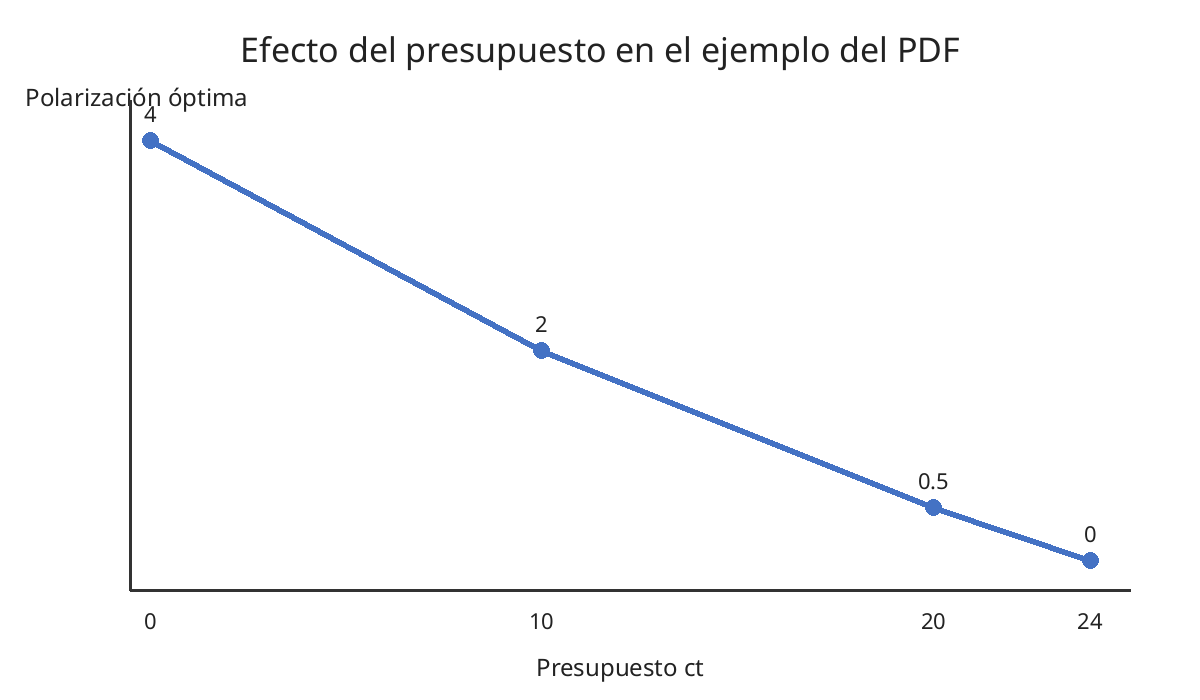
\includegraphics[width=\dimexpr\linewidth-0.20cm\relax,height=4.25cm,keepaspectratio]{presupuesto_polarizacion.png}\end{beamercolorbox}
      \vspace{0.18cm}\centering\pill[teal]{6.6cm}{$ct$: 0 $\to$ 24 · polarización: 4 $\to$ 0}
    \end{column}
    \begin{column}{0.49\textwidth}
      \begin{beamercolorbox}[wd=\dimexpr\linewidth-0.20cm\relax,sep=0.10cm,rounded=true]{card}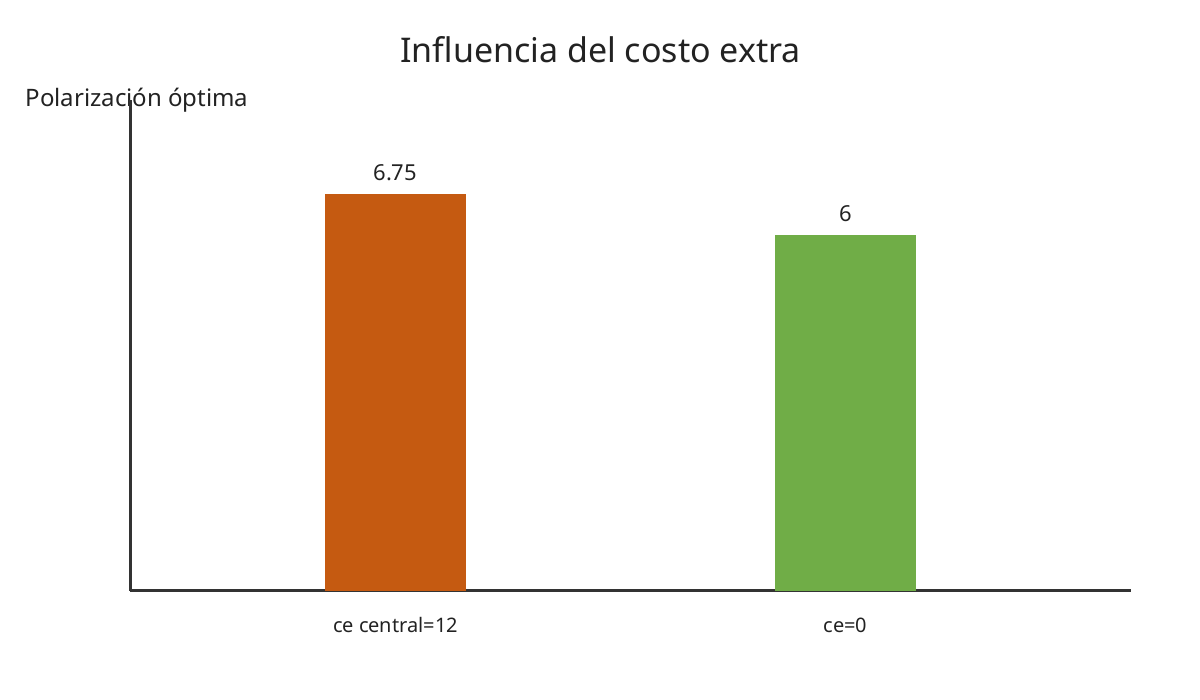
\includegraphics[width=\dimexpr\linewidth-0.20cm\relax,height=4.25cm,keepaspectratio]{impacto_costo_extra.png}\end{beamercolorbox}
      \vspace{0.18cm}\centering\pill[amber]{6.6cm}{$ce$: 12 $\to$ 0 · polarización: 6.75 $\to$ 6}
    \end{column}
  \end{columns}
\end{frame}

% 12. Eficiencia
\speaker{Juan Esteban Rodriguez Valencia}{8:10--9:00}
\begin{frame}{Branch and Bound: ramificar, acotar y podar}
  \framesubtitle{Tamaño: $m^2$ variables $x$ + $m^2$ auxiliares $q$ + $m$ binarias $z$}
  \begin{columns}[T,onlytextwidth]
    \begin{column}{0.50\textwidth}
      \begin{beamercolorbox}[wd=\dimexpr\linewidth-0.20cm\relax,sep=0.10cm,rounded=true]{card}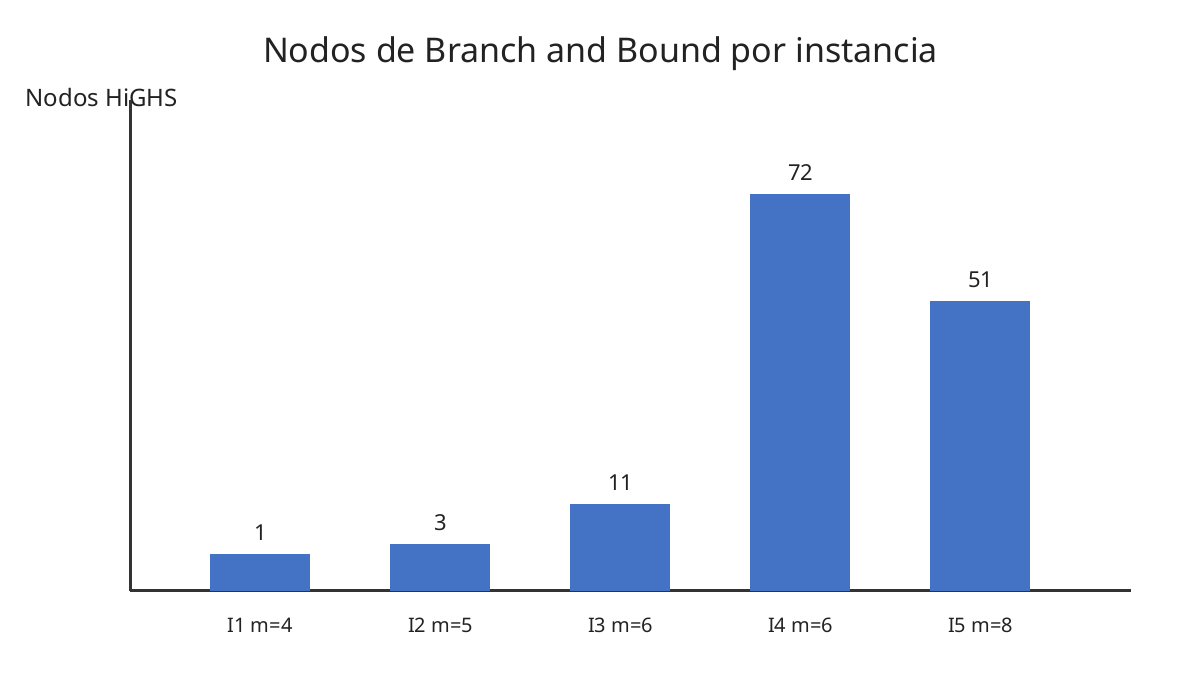
\includegraphics[width=\dimexpr\linewidth-0.20cm\relax,height=4.30cm,keepaspectratio]{nodos_instancias.png}\end{beamercolorbox}
    \end{column}
    \begin{column}{0.48\textwidth}
      \scriptsize
      \begin{beamercolorbox}[wd=\linewidth,sep=0.18cm,rounded=true]{card}
        {\color{blue}\bfseries 1 · RAMIFICACIÓN}\quad Variable fraccionaria $\to$ dos subproblemas.\par\vspace{0.16cm}
        {\color{red}\bfseries 2 · PODA INFACTIBLE}\quad La relajación lineal no tiene solución.\par\vspace{0.16cm}
        {\color{amber}\bfseries 3 · PODA POR COTA}\quad En minimización, $LB\geq UB$: no mejora al incumbente.\par\vspace{0.16cm}
        {\color{green}\bfseries 4 · CIERRE INTEGRAL}\quad Si una solución entera mejora al incumbente, actualiza $UB$.
      \end{beamercolorbox}\vspace{0.18cm}
      \begin{beamercolorbox}[wd=\linewidth,sep=0.14cm,center,rounded=true]{cardalt}
        \bfseries HiGHS: 1 nodo · Chuffed: 225 nodos\par{\color{muted}\scriptsize Misma instancia; estrategias distintas}
      \end{beamercolorbox}
    \end{column}
  \end{columns}
\end{frame}

% 13. Prueba 1
\sectiontag{4 · PRUEBAS Y CONCLUSIONES}
\speaker{Estiven Andres Martinez Granados}{9:00--10:15}
\begin{frame}{Prueba 1 · ejemplo del enunciado}
  \framesubtitle{Cargar MPL · generar DZN · resolver con HiGHS · revisar 7 verificaciones}
  \begin{columns}[c,onlytextwidth]
    \begin{column}{0.31\textwidth}\centering\pill[blue]{\linewidth}{INICIAL · [12, 4, 0, 4, 0]}\end{column}
    \begin{column}{0.08\textwidth}\centering{\color{amber}\Large$\longrightarrow$}\end{column}
    \begin{column}{0.34\textwidth}\centering\pill[green]{\linewidth}{FINAL · [18, 2, 0, 0, 0]}\end{column}
  \end{columns}\vspace{0.03cm}
  \centering\bfseries\large $4\times(2\to1)$ \quad·\quad $2\times(4\to1)$ \quad·\quad $2\times(4\to2)$
  \vspace{0.04cm}
  \begin{columns}[T,onlytextwidth]
    \begin{column}{0.24\textwidth}\metric{19.2 / 20}{costo}{amber}\end{column}
    \begin{column}{0.24\textwidth}\metric{14 / 18}{movimientos}{blue}\end{column}
    \begin{column}{0.24\textwidth}\metric{0}{mediana}{teal}\end{column}
    \begin{column}{0.24\textwidth}\metric{0.5}{polarización}{green}\end{column}
  \end{columns}\vspace{0.03cm}
  \begin{columns}[T,onlytextwidth]
    \begin{column}{0.49\textwidth}\infocard{\linewidth}{teal}{COMPROBACIÓN}{Costo: $4.8+9.6+4.8=19.2$\par Movimientos: $4+6+4=14$}\end{column}
    \begin{column}{0.49\textwidth}\infocard{\linewidth}{green}{MEJORA CERTIFICADA}{Polarización: $4\to0.5$ ($-87.5\%$)\par 447 distribuciones factibles enumeradas}\end{column}
  \end{columns}\vspace{0.02cm}
  \centering\pill[green]{9.8cm}{DOMINIO · BALANCE · PRESUPUESTO · $maxM$ · MEDIANA}
\end{frame}

% 14. Prueba 2
\speaker{Estiven Andres Martinez Granados}{10:15--11:05}
\begin{frame}{Prueba 2 · consenso alcanzable}
  \framesubtitle{Tres personas recorren dos posiciones y consumen todo $maxM$}
  \begin{columns}[c,onlytextwidth]
    \begin{column}{0.28\textwidth}\centering\pill[blue]{\linewidth}{INICIAL · [7, 0, 3, 0]}\end{column}
    \begin{column}{0.07\textwidth}\centering{\color{amber}\Large$\longrightarrow$}\end{column}
    \begin{column}{0.28\textwidth}\centering\pill[green]{\linewidth}{FINAL · [10, 0, 0, 0]}\end{column}
    \begin{column}{0.28\textwidth}\centering\pill[teal]{\linewidth}{3 PERSONAS · $3\to1$}\end{column}
  \end{columns}\vspace{0.40cm}
  \begin{columns}[T,onlytextwidth]
    \begin{column}{0.32\textwidth}\infocard{\linewidth}{amber}{PRESUPUESTO}{$3\times$ costo efectivo\par $=11.7\leq12$}\end{column}
    \begin{column}{0.32\textwidth}\infocard{\linewidth}{blue}{MOVIMIENTOS}{$3\times|1-3|$\par $=6=maxM$}\end{column}
    \begin{column}{0.32\textwidth}\infocard{\linewidth}{green}{OBJETIVO}{$10\times|0-0|$\par $=0$}\end{column}
  \end{columns}\vspace{0.45cm}
  \begin{beamercolorbox}[wd=\linewidth,sep=0.28cm,rounded=true]{cardalt}
    \begin{columns}[c,onlytextwidth]
      \begin{column}{0.20\textwidth}{\color{green}\bfseries\large CONSENSO}\end{column}
      \begin{column}{0.76\textwidth}{\centering\bfseries Es posible solo si una concentración completa respeta $ct$ y $maxM$ simultáneamente.}\end{column}
    \end{columns}
  \end{beamercolorbox}
\end{frame}

% 15. Conclusiones
\speaker{Estiven Andres Martinez Granados}{11:05--12:00}
\begin{frame}{Qué demostramos}
  \framesubtitle{Movimientos factibles, auditables y óptimos para las instancias evaluadas}
  \small
  \begin{columns}[T,onlytextwidth]
    \begin{column}{0.32\textwidth}\infocard{\linewidth}{teal}{01 · Modelo exacto}{IP/PLE con mediana linealizada}\end{column}
    \begin{column}{0.32\textwidth}\infocard{\linewidth}{amber}{02 · Factibilidad}{Población, $ct$ y $maxM$ separados}\end{column}
    \begin{column}{0.32\textwidth}\infocard{\linewidth}{blue}{03 · Precisión}{Escalamiento entero de decimales}\end{column}
  \end{columns}\vspace{0.16cm}
  \begin{columns}[T,onlytextwidth]
    \begin{column}{0.49\textwidth}\infocard{\linewidth}{green}{04 · Evidencia}{30/30 entradas verificadas}\end{column}
    \begin{column}{0.49\textwidth}\infocard{\linewidth}{red}{05 · Límite}{Crecimiento cuadrático en $m$}\end{column}
  \end{columns}\vspace{0.22cm}
  \begin{beamercolorbox}[wd=\linewidth,sep=0.30cm,rounded=true]{tablehead}
    \begin{columns}[c,onlytextwidth]
      \begin{column}{0.18\textwidth}{\bfseries\Large MinPol}\end{column}
      \begin{column}{0.78\textwidth}{\centering\bfseries Brecha 0\% · verificación independiente · resultados reproducibles}\end{column}
    \end{columns}
  \end{beamercolorbox}\vspace{0.20cm}
  \centering{\color{green}\bfseries\Large Muchas gracias}
\end{frame}

\end{document}
